\chapter{Modelación para la simulación de enfermedades transmitidas por vectores}\label{chapter:proposal}
\section{Vectores en la naturaleza}
Un vector es un organismo vivo, como un insecto o artrópodo, que puede transmitir un agente 
infeccioso, como un virus, una bacteria o un parásito, de un huésped infectado a un huésped 
susceptible. Los vectores pueden actuar como intermediarios en la transmisión de enfermedades, 
ya sea mecánicamente, a través de la contaminación de alimentos o superficies con el agente 
infeccioso, o biológicamente, cuando el agente infeccioso se replica y multiplica dentro del 
vector antes de ser transmitido a un nuevo huésped. Los vectores son una parte integral de la 
epidemiología de muchas enfermedades infecciosas y desempeñan un papel crucial en su mantenimiento 
y propagación.\autocite{Reisen2010}

Según la OMS, las enfermedades airborne (arthropod-borne)\footnote{enfermedades infecciosas que 
se transmiten a través de la picadura de artrópodos, como mosquitos, garrapatas, pulgas o moscas.} 
representan 17 por ciento del total de las enfermedades infecciosas en el mundo, con 1,000 millones 
de casos y un millón de defunciones anuales \autocite{OMS2020}. Los vectores biológicos más 
comunes son los insectos hematófagos que al alimentarse de la sangre de un portador infectado, 
ingieren microorganismos patógenos que posteriormente inoculan a otro individuo.

\textbf{Características generales de los vectores:}\autocite{OMS2020}
\begin{enumerate}
    \item Especies específicas: Los vectores suelen ser especies específicas de insectos, 
    artrópodos u otros organismos. Por ejemplo, los mosquitos, las garrapatas, las pulgas y los 
    flebótomos son ejemplos comunes de vectores. 
    \item Capacidad de transmitir enfermedades: Los vectores tienen la capacidad de transmitir 
    agentes patógenos, como virus, bacterias o parásitos, de un huésped infectado a un huésped 
    susceptible. Esto puede ocurrir a través de la picadura o el contacto con el vector.
    \item Dependencia de los huéspedes: Los vectores dependen de la sangre u otros recursos de 
    sus huéspedes para alimentarse y reproducirse. Por lo tanto, su presencia y actividad están 
    estrechamente relacionadas con la disponibilidad de los huéspedes adecuados.
\end{enumerate}
\subsection{Enfermedades Transmitidas por Vectores (ETV)}
Entre las ETV que han aumentado en las últimas décadas están el 
paludismo o malaria, la fiebre hemorrágica por dengue, la esquistosomiasis, la tripanosomiasis americana 
o enfermedad de Chagas, la tripanosomiasis africana o enfermedad del sueño, la leishmaniasis, la fiebre 
amarilla, la encefalitis japonesa, la fiebre por zika  y la fiebre por chikungunya. Otras ETV menos frecuentes 
son la borreliosis o enfermedad de  Lyme y la enfermedad por el  virus del oeste del Nilo.\autocite{Torres2020}\\

\begin{figure}[htb]
    \centering
    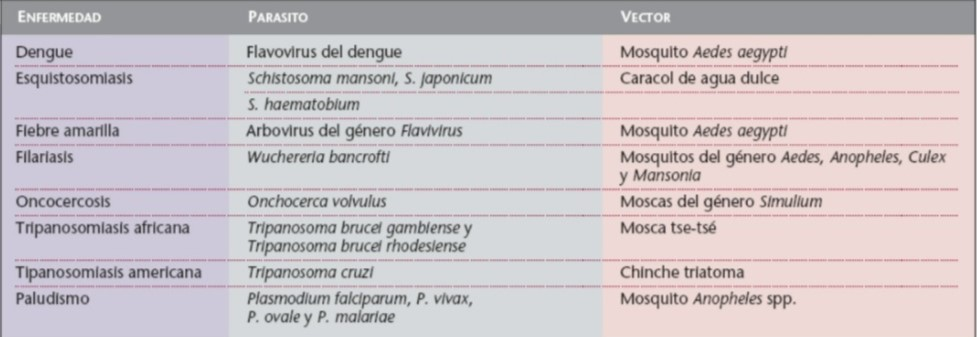
\includegraphics[width=1\textwidth]{Graphics/EnfVec.jpeg}
    \caption{Algunas enfermedades transmitidas por vectores.\autocite{Tercero2008}}
\end{figure}

La distribución de las ETV está vinculada a una serie de factores complejos 
de naturaleza demográfica, ecológica, medioambiental y social. Estos factores incluyen:
\begin{enumerate}
    \item El fenómeno del calentamiento global y el consiguiente cambio climático, que permite la adaptación de los vectores a nuevas altitudes y la propagación de patógenos en regiones previamente no afectadas.
    \item La sobrepoblación y el hacinamiento en áreas específicas, lo cual propicia un aumento en la presencia de vectores y hospederos susceptibles, como perros y gatos.
    \item La densidad de población de los artrópodos vectores y la diversidad de especies presentes en un área determinada.
    \item La falta de medidas adecuadas de higiene a nivel personal, en viviendas y en comunidades.
    \item El incremento en la frecuencia y distancia de los viajes internacionales.
    \item La existencia de marginación, pobreza y urbanización descontrolada.
\end{enumerate}

Actualmente, la enfermedad transmitida por vector con mayor crecimiento mundial es el dengue. 
Al igual que el virus del dengue, el del Zika, el chikungunya y la fiebre amarilla son transmitidos 
por los mosquitos Aedes aegypti y Aedes albopticus. Más de 3900 millones de personas en más de 129 
países corren el riesgo de contraer dengue, y se estima que cada año se registran 96 millones de casos 
sintomáticos y 40 000 muertes.\autocite{OMS2020}

\section{Dengue}
El dengue es una enfermedad viral transmitida por mosquitos que representa un desafío significativo 
para la salud pública a nivel mundial. Esta enfermedad se encuentra principalmente en regiones tropicales 
y subtropicales, pero su alcance se ha extendido durante las últimas décadas, llegando a afectar a más de 100 
países. El virus del Dengue está formado por cuatro serotipos: dengue1, dengue2, dengue3 y dengue4. La 
infección humana por un serotipo produce inmunidad para toda la vida contra la reinfección por ese serotipo, 
pero el individuo queda susceptible a los otros tres. \autocite{Simmons2012}

Una vez que una persona es picada por un mosquito infectado, se produce un período de incubación en esta, que puede 
durar de 5 a 7 días, luego de esto aparecen los primeros síntomas. El humano se encuentra enfermo aproximadamente
durante 7 o 15 días. En el momento en el que surgen los primeros síntomas comienza el período crítico de 
transmisión. Si en este intervalo de tiempo un mosquito pica a esa persona, entonces tiene una probabilidad 
alta de adquirir la enferemedad y luego de 8 a 12 días el virus se aloja en las glándulas salibales del mosquito
y es en esta etapa en que el mosquito es capaz de transmitir la enfermedad. \autocite{OMS2023}

Una de las características más preocupantes del Dengue es su capacidad para causar una amplia gama de síntomas, 
desde una fiebre leve hasta formas más preocupantes que pueden poner en peligro la vida. La forma grave de la 
enfermedad, conocida como fiebre hemorrágica del dengue, puede producir hemorragias internas, 
disfunción orgánica y shock. Esta forma afecta principalmente a niños pequeños, 
adultos mayores y personas con sistemas inmunológicos debilitados.\\

\textbf{Síntomas del Dengue:}\autocite{OMS2023}
\begin{enumerate}
    \item Fibre alta ($40^{\circ}$C).
    \item Dolores de cabeza.
    \item Dolor detrás de los ojos.
    \item Náuseas
    \item Vómitos
    \item Rash
\end{enumerate}

El mosquito aedes aegypti es el vector del Dengue. El ciclo de vida de un mosquito es aproximadamente entre 4 y 
8 semanas y ocurre en varias etapas, huevo, larva, pupa y adulto. Los que transmiten la enfermedad son los mosquitos
hembras adultos. Estas necesitan de sangre para desarrollar los huevos y pueden volar hasta 3 kilómetros con 
el objetivo de encontrar un lugar para ponerlos, aunque no se espera que vuelen más de 100 metros del sitio 
donde viven.

\section{Modelación del entorno}
Lo primero que se debe crear y modelar para simular cómo ocurre la propagación de enfermedades es el 
entorno en que ocurrirá la misma. La idea de este trabajo es lograr representar la realidad de la sociedad
y para esto se entiende que existen parámetros a desarrollar: las relaciones personales, los lugares y el comportamiento
de las personas.

\subsection{Localizaciones}
En la actualidad la mayoría de las personas tienen un programa de vida definido, es decir, una persona $x$ tiene una 
vivienda, un centro de trabajo y otros lugares a los que asiste por determinadas circunstancias; por lo que
para representar la sociedad, es necesario según se entiende, modelar estos lugares.

Para esto, los lugares son considerados un objeto en nuestro proyecto. Se entiende por lugar una localización en
la cual pueden asistir personas y vectores y además este puede brindar cierto recurso. Por ejemplo: ¿cómo se
representaría un mercado en nuestra simulación?, un mercado posee una capacidad para albergar personas y vectores 
y además brinda la posibilidad de obtener comida, aseo, entre otros.

\textbf{Localizaciones relevantes a representar:}
\begin{enumerate}
    \item Casas: representa un hogar familiar.
    \item Hospitales: indica un centro de atención médica.
    \item Centros de trabajo: hace referencia a todo lugar laboral, pero no significa que si una persona está en este, se encuentra trabajando, por ejemplo: en una escuela (centro de trabajo) hay personas que no están trabajando como los niños.
    \item Mercados.
\end{enumerate}

Este tipo de localizaciones nos permite abarcar toda construcción en la que pueden relacionarce las personas, pues
el tipo de lugar $"Centro$ $de$ $Trabajo"$ sirve de comodín en nuestra simulación.

\subsection{Personas}
Una de las herramientas conocidas para describir relaciones entre agentes son los grafos \autocite{Newman2003}. Un grafo
es un par ordenado $G = (V,E)$ donde $V$ es un conjunto no vacío de nodos y $E$ es un conjunto de pares 
no ordenados de aristas.

\begin{center}
    $G=(V,E)$ tal que:\\
    \begin{enumerate}
        \item $V$ = $\lbrace$ $v_{1}$, $v_{2}$, $v_{3}$, ..., $v_{n}$ $\rbrace$ es un conjunto finito de vértices.
        \item $E$ = $\lbrace$($v_{i}$,$v_{j}$)|$v_{i}$, $v_{j}$ $\in$ $V$ $\rbrace$  es un conjunto de pares no ordenados de vértices que representan las aristas del grafo.
    \end{enumerate}
\end{center}

En nuestro proyecto se construye un grafo que representa la relación $\textbf{ser familia}$ y la relación \textbf{ser conocidos}, brindando
la posibilidad de escoger la probabilidad con la que se genere una arista entre dos nodos y la cantidad de nodos a crear. 
En este, un nodo $v_{i}$ representa a la persona $i$ de la simulación y una arista ($v_{i}$, $v_{j}$) simboliza,
o bien la relación $i$ $\rightarrow$ $j$ son familiares, o son conocidos, es decir no existe un tipo de arista para cada
tipo de relación. ¿Cómo se identifica entonces si la arista ($v_{i}$, $v_{j}$) representa la relación 
ser familia o la relación conocidos?

Para esto se realiza un proceso estocástico que ocurre una sola vez (al inicio de la simulación), el cual consiste 
en escoger de manera aleatoria el conjunto $C$ que se define a continuación.
\begin{center}
    Sea $G = (V,E)$ un grafo de nuestra simulación.\\
    Sea $H \subset V$ tal que $v_{i} \in H \Leftrightarrow \forall v_{j} \in H, (v_{i},v_{j}) \in E$\\
    Sea $C = \lbrace H_{1}, H_{2}, ..., H_{l} \rbrace$,$\forall i$ $H_{i} \subset V$ tal que si $v_{j} \in H_{i} \Rightarrow v_{j} \notin H_{k}$ $\forall k \neq i$\\
\end{center}

Entonces las relaciones están definidas de la siguiente forma:
\begin{center}
    $\forall i,j$ $(v_{i}, v_{j}) \in E$ representa la relación ser familia  $\Leftrightarrow \exists k$ tal que $v_{i}, v_{j} \in H_{k}$, $H_{k} \in C$.\\
    Si $v_{i} \in H_{k}, v_{j} \notin H_{k}$, $H_{k} \in C$ y $\exists (v_{i}, v_{j}) \Rightarrow$ la arista $(v_{i}, v_{j})$  representa
    la relación ser conocidos.
\end{center}


\begin{figure}[htb]
    \centering
    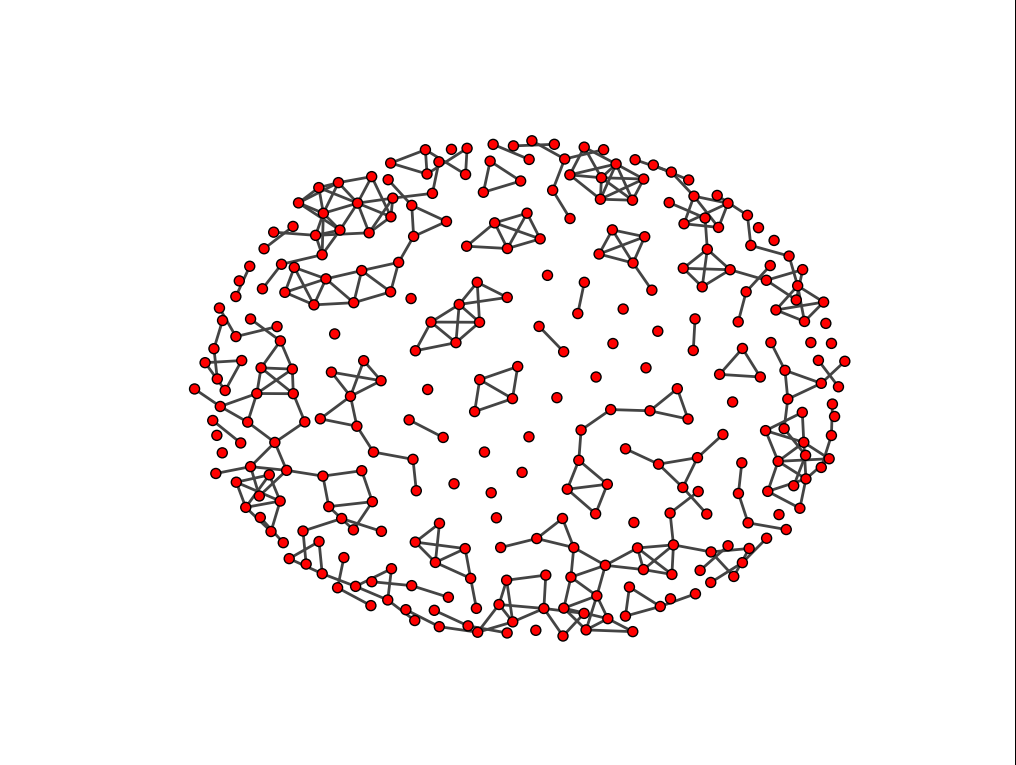
\includegraphics[width=0.8\textwidth]{Graphics/Grafo_Pers.png}
    \caption{Ejemplo de grafo de relaciones personales generados por el modelo. Personas: 300, probabilidad de arista: 0.05}
\end{figure}

\begin{figure}
    \centering
    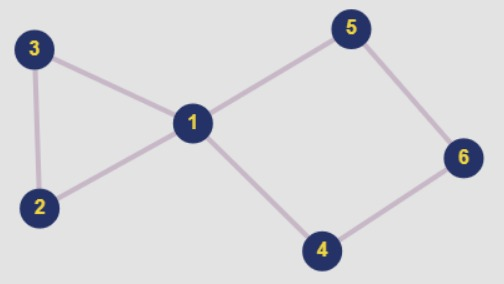
\includegraphics[width=0.3\textwidth]{Graphics/Grafo_Familias.jpeg}
    \caption{Ejemplo de grafo de relaciones personales para ilustrar.}
\end{figure}

En la figura 2.3 se observa un posible grafo generado. En este grafo los posibles conjuntos $H$ serían: 
$H_{1} = (1,2)$; $H_{2}=(1,3)$; $H_{3}=(2,3)$; $H_{4} = (1,2,3)$; $H_{5} = (1,5)$; $H_{6}=(1,4)$; $H_{7} = (4,6)$; $H_{8} = (5,6)$ y por último tantos conjuntos $H$ como nodos haya, es decir
todos los posibles cliques del grafo. De estos conjuntos se seleccionarían aleatoriamente algunos para formar el conjunto $C$;
por ejemplo $C = \lbrace H_{4}, H_{7}, H_{13}$\footnote{A partir de $H_{8}$ comienzan los conjuntos que representan a cada nodo, por tanto $H_{13}$ hace referencia al nodo $5$} $\rbrace$; y los nodos que están en los $H_{i} \in C$ serían considerados
familias entre ellos.

Las personas, en el curso de la realización de sus actividades diarias (como el trabajo, el estudio o las compras),
se desplazan entre varios lugares, exponiéndose a agentes infecciosos dentro de estos lugares y transportando las
enfermedades. Para lograr representar y modelar estos procesos se genera una red de contactos sociales que puede
ser vista como un grafo bipartito, en el cual el conjunto $A$ está compuesto por todas las personas de la simulación
y el conjunto $B$ por todas las localizaciones. Las aristas en este grafo son dirigidas y representan 
el lugar en donde se encuentra la persona.


\begin{figure}[htb]
    \centering
    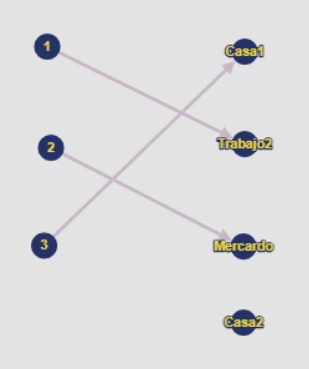
\includegraphics[width=0.3\textwidth]{Graphics/Grafo_Loc_Pers.jpeg}
    \caption{Ejemplo de grafo que representa a la red de contactos sociales.}
\end{figure}

\begin{center}
    Sea $G = (V,E)$ grafo dirigido. 
    $\forall i,j$ si $(v_i,v_j) \in E \Rightarrow$ la persona $v_i$ se encuentra en el lugar $v_j$ 
\end{center}

El grafo definido anteriormente es un grafo dinámico, es decir varía en dependencia del lugar en donde se encuentre
una persona, pues al decidir un agente ir a otro lugar, se elimina la arista que antes este tenía en el grafo y se 
añade la nueva arista, la cual representa el lugar en donde se encuentra en el momento. (Los vértices que representan
personas tienen $outdegree$\footnote{Hace referencia a la cantidad de aristas que salen del vértice en cuestión, 
se mantiene el término en inglés pues es lo usado en el ámbito científico} igual a 1)

\subsection{Vectores}
Los vectores son seres vivos al igual que las personas, pero a diferencia de ellas, estos poseen menos movilidad que las
personas. Para la representación de los vectores en el modelo no se tiene en cuenta la relación que 
poseen entre ellos pues se entiende que es suficiente con las relaciones de las personas para lograr simular 
la propagación de una enfermedad.

Los mosquitos como bien se mencionó anteriormente se establecen en un lugar y poco o nada se mueven de 
sus alrededores, por tanto, se decidió que los vectores en nuestra simulación no tuviesen la capacidad de moverse por
las localizaciones como las personas ya que esto nos acerca más a lo que ocurre en la realidad.

Los vectores se modelan con la posibilidad de picar y de infectarse. Estos, según mecanismos estocásticos,
deciden si picar o no y teniendo en cuenta el nivel de infección de la persona y la susceptibilidad del mismo este
se infecta o no. También poseen un parámetro que representa la probabilidad de infectarse debido a una picada, mientras
mayor sea el valor de dicho parámetro, más probable será que el mosquito se infecte si pica a una persona enferma.

\begin{figure}[htb]
    \centering
    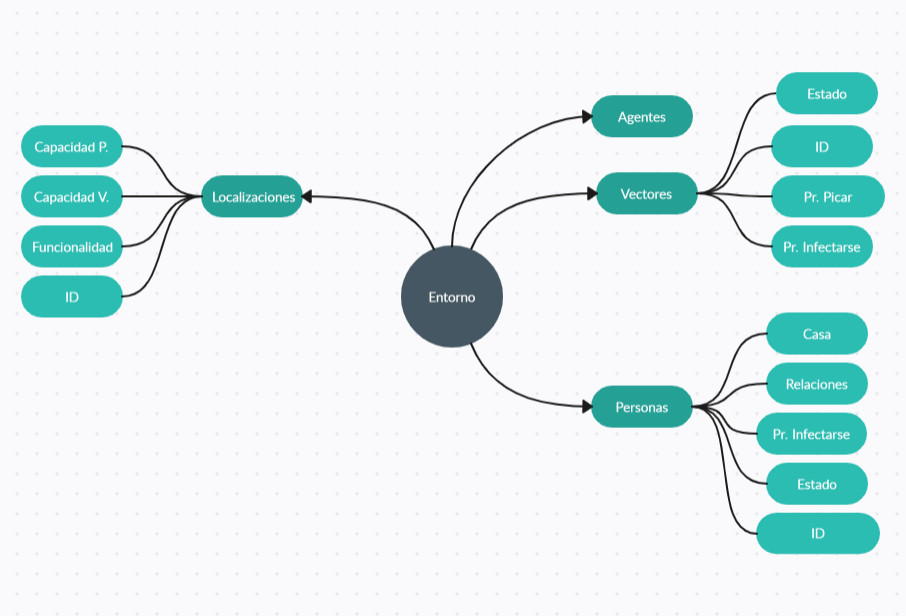
\includegraphics[width=0.9\textwidth]{Graphics/Pers_Loc_Vec.png}
    \caption{Esquema que representa el entorno modelado.}
\end{figure}
En la figura 2.5 se observa como se encuentra modelado el entorno de la simulación. Existen unos agentes que son las
personas y los vectores, los cuales poseen ciertas características y estos interactúan con las localizaciones para
cumplir sus propósitos; el de las personas trabajar y socializar y el de los vectores alimentarse, logrando así
acercarnos a un modelo que representa de forma precisa cómo se propaga un efermedad transmitida por vectores.

\section{Interacción de los agentes con el entorno}
Una vez diseñado el entorno y los agentes que conviven en el mismo, se abre paso al siguiente aspecto:
¿Cómo interactúan entre sí? La interacción entre los agentes y su medio es esencial para comprender 
cómo se desarrollará y evolucionará el sistema en cuestión.\\
Existen muchas formas de desarrollar las interacciones, dependiendo del contexto y los objetivos establecidos
para los agentes. Pueden ser directas, donde los agentes interactúan entre sí de manera mutuamente perceptible,
indirectas, donde los agentes influyen en el entorno, y a su vez, el entorno afecta a la forma en que estos se 
comportan y un híbrido en el que los agentes según sus decisiones afectan al medio y a otros agentes, y también, 
el entorno los afecta.\\
Las interacciones pueden estar basadas en reglas predefinidas, donde se establecen normas, objetivos y una serie
de comportamientos específicos, o pueden ser adaptativas, donde los agentes aprenden a medida que intercambian con
el entorno, obteniendo retroalimentación del mismo, para modificar su comportamiento.\\
Una herramienta computacional que brinda la posibilidad de crear agentes con cierta inteligencia para manejar
sus decisiones son los Mapas Cognitivos Difusos\footnote{FCM por sus siglas en inglés}. Para el diseño de un $FCM$ es necesario definir los 
conceptos que este agrupará, así como las categorías de conceptos.\\
¿Qué son los conjuntos difusos? Zadeh en \autocite{Zadeh1965} da respuesta a esta interrogante de la siguiente forma.
\begin{center}
    Sea $X$ un espacio de puntos en los que los elementos de $X$ son $x$. $X = \lbrace x \rbrace$
\end{center}
Un conjunto difuso $A$ en $X$ es caracterizado por una función de membresía $f_A(x)$ que asocia a cada punto en 
$X$ un valor real en el intervalo $[0, 1]$ con el valor de $f_A(x)$ en $x$ representando el 
grado de membresía de $x$ en $A$, tal que mientras más cerca el valor de $f_A(x)$ a la unidad más alto es 
el grado de membresía de $x$ en $A$. Pongamos un ejemplo representado en \autocite{Zadeh1965}.\\
Sea $X$ el conjunto de los números reales $R$ y sea $A$ un conjunto difuso de los números que son mucho mayores que 1.
La función $f_A(X)$ podría tener ciertos valores representativos como: $f_A(0) = 0$, $f_A(1) = 0$,
$f_A(5) = 0.01$, $f_A(10) = 0.2$, $f_A(100) = 0.95$, $f_A(500) = 1$.

Es importante notar que cuando el conjunto $X$ es un conjunto contable la función de membresía es parecida a una 
función de probabilidad (o parecido a la función de densidad cuando $X$ es continuo), evidentemente existen
diferencias entre estos conceptos las cuales son especificadas por Zadeh en \autocite{Zadeh1965}.

% \textbf{Algunas definiciones de conjuntos difusos:}\autocite{Zadeh1965}\\
% \begin{itemize}
%     \item Se dice que dos conjuntos difusos $A$ y $B$ son iguales, $\Leftrightarrow$ $f_A(X) = f_B(x)$ $\forall x$ en $X$.
%     \item Un conjunto difuso $A$ es vacío $\Leftrightarrow$ $f_A(x) = 0$ $\forall x$ en $X$.
%     \item El complemento de un conjunto difuso $A$ es $A'$ y es definido de la siguiente forma: $f_{A'} = 1 - f_A$.
%     \item $A \subset B \Leftrightarrow f_A \leqq f_B$
% \end{itemize}

En el Capítulo $"Estado$ $del$ $Arte"$ se realiza un acercamiento a la posibilidad de crear un $FCM$ con tres clases de 
conceptos; $Percepciones$, $Sentimientos$ y $Acciones$. Cada clase tiene una serie de conceptos que posibilitan la 
interacción entre clases.\\
Al separar los conceptos se comienza a ver el grafo del $FCM$ como un grafo bipartito, en el cual el conjunto $A$
se encuentra formado por los conceptos de las clases $Percepciones$ y $Acciones$ y el conjunto $B$ por la clase
$Sentimientos$. Entonces, surge una interrogante, ¿cuál sería el flujo a seguir de este $FCM$ para que los agentes
decidan una acción u otra?\\
La idea es la siguiente, un agente percibe un estado del entorno, este estado, provoca un sentimiento en el agente
y, a su vez, este sentimiento provoca una acción.
\begin{center}
    $Percepciones \rightarrow Sentimientos \rightarrow Acciones$\\
\end{center}

A medida que va cambiando el entorno, va cambiando la perspectiva del agente, esta afecta a los sentimientos del mismo 
y con esto cambia la probabilidad de efectuar una acción u otra. Por tanto, el tipo de relación utilizada en este $FCM$
es híbrida, cada pequeño cambio, ya sea, en el entorno, o en el mapa cognitivo difuso de un agente, afecta a los conceptos
del $FCM$ de los agentes restantes.

\section{Conceptos (Personas)}
\subsection{Perspectiva}
Para la sección de los conceptos de percepción se observa que una idea útil es que, para cada concepto, se crea su contrapuesto
como concepto, por ejemplo, si se definiese el concepto $"cercan$í$a de hospital"$, entonces sería útil definir el concepto
$"lejan$í$a de hospital"$ pues las posibles acciones a ejecutar se beneficiarían por uno y se perjudicarían por el otro,
añadiendo facilidad a la decisión del agente.\\
\\
\textbf{Conceptos definidos para la categoría Perspectiva:}
\begin{itemize}
    \item Personas enfermas alta. (1.4)
    \item Personas enfermas baja. (1.4)
    \item Comida alta. (1.5)
    \item Comida baja. (1.5)
    \item Energía alta. (3)
    \item Energía baja. (3)
    \item Dinero alto. (1.5)
    \item Dinero bajo. (1.5)
    \item Enfermedad alta. (3.2)
    \item Enfermedad baja. (3.2)
\end{itemize}

Cada concepto en esta categoría, tiene un parámetro que representa cuán grande es el intervalo que se considera para darle un valor en la 
$fuzzificaci$ó$n$ entre $(0,1)$ al concepto\footnote{el número que se encuentra entre paréntesis al lado del concepto}, en caso 
de que sea menor o mayor a los límites del intervalo, su valor final es $0$ o $1$ respectivamente, pero, ¿por qué
se realiza este procedimiento?

La idea de implentar de esta forma esta categoría es para $fuzzificar$ teniendo en cuenta lo que se percibe 
del entorno. El valor de este parámetro por concepto nunca cambia, entonces surge la interrogante siguiente: 
¿cómo modelar que la perspectiva del entorno varía? Este valor pasa por un proceso en el cual se toman variables que sí
cambian en el entorno y se utiliza el mismo para $fuzzificar$ el valor del concepto, el cual es distinto al parámetro 
representado en la lista anterior.

El proceso de $fuzzificaci$ó$n$ es distinto para cada concepto, pero por regla general se sigue la siguiente idea:\\
\begin{enumerate}
    \item Se toma un valor del entorno del agente que tenga relación con el concepto a $fuzzificar$, llamémosle $variable$ $de$ $fuzzificaci$ó$n$.
    \item Se obtiene un intervalo de valores utilizando el parámetro del concepto, llamémosle $intervalo$ $de$ $fuzzificaci$ó$n$.
    \item Se compara la $variable$ $de$ $fuzzificaci$ó$n$ con los extremos del $intervalo$ $de$ $fuzzificaci$ó$n$, en el caso de encontrarse incluida en este se decide si es más importante que se encuentre cerca del máximo o del mínimo del $intervalo$ $de$ $fuzzificaci$ó$n$ y se $fuzzifica$ de acuerdo al intervalo, teniendo en cuenta cual extremo es considerado $1$ y cual $0$ en el proceso de $fuzzificaci$ó$n$.
\end{enumerate}

\begin{center}
    Sea $v$ la $variable$ $de$ $fuzzificaci$ó$n$.\\
    Sea $(i_0, i_1)$ el $intervalo$ $de$ $fuzzificaci$ó$n$.\\
    Sea $r$ el resultado del proceso de $fuzzificaci$ó$n$.\\
    Sea $inv$ una variable booleana, tal que: $if$ $inv = True, v \geq i_1 \Rightarrow r = 1$ , $if$ $inv = False, v \leq i_0 \Rightarrow r = 1$\\
\end{center}
    Cuando $v$ se encuentra dentro del intervalo ocurre lo siguiente:
\begin{center}
    $if$ $inv = True$ $\Rightarrow$ $r = \frac{v - i_0}{i_1 - i_0}$\\
    $if$ $inv = False$ $\Rightarrow$ $r = \frac{i_1 - v}{i_1 - i_0}$
\end{center}

La combinación de valores en estos conceptos, o el valor de un concepto por sí mismo, afecta al valor que toma algún
concepto en la categoría $Sentimientos$.

\subsection{Sentimientos}
En esta categoría se tienen en cuenta los sentimientos básicos de un ser humano y los que mejor se adaptaban para
representar la movilidad de los mismos.\\
\\
\textbf{Conceptos definidos para la categoría Sentimientos:}
\begin{itemize}
    \item Miedo.
    \item Hambre.
    \item Necesidad.
    \item Enfermedad.
    \item Indiferencia.
    \item Cansancio.
\end{itemize}

\subsection{Acciones}
Se definen las acciones fundamentales que modelan el comportamiento de una persona en un ambiente epidémico.\\
\\
\textbf{Conceptos definidos para la categoría Acciones:}
\begin{itemize}
    \item Ir a trabajar.
    \item Ir al mercado.
    \item Ir al hospital.
    \item Caminar.
    \item Estudiar.
    \item Descansar.
    \item Prevenir.
\end{itemize}

\begin{figure}[htb]
    \centering
    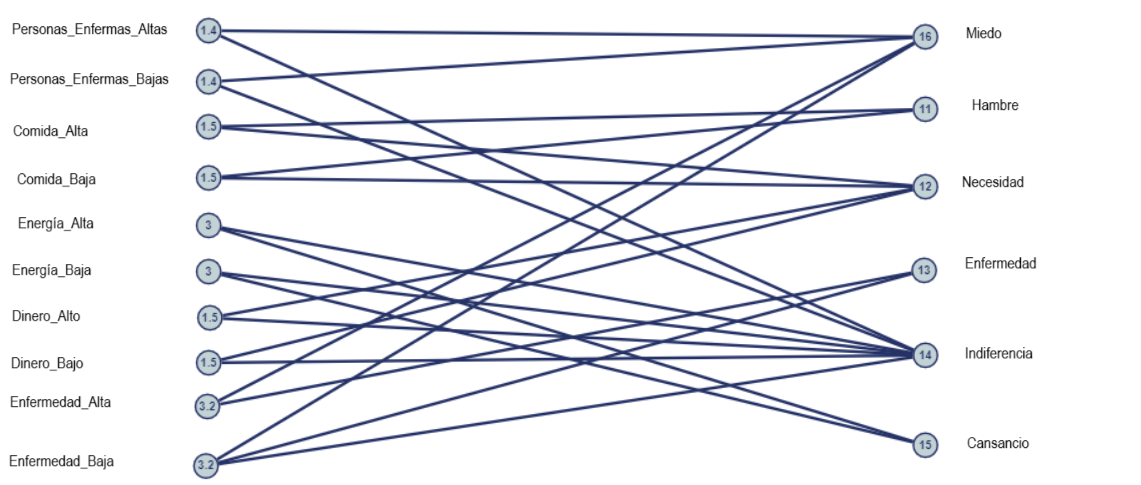
\includegraphics[width=0.9\textwidth]{Graphics/Grafo_Pers-Sent.png}
    \caption{Grafo que representa las relaciones entre los nodos de $percepci$ó$n$ y $sentimientos$ del $FCM$ inicial de cada persona}
\end{figure}
\newpage
Los nodos $percepci$ó$n$ representados a la izquierda en la figura 2.6 poseen unos pesos. Estos son utilizados
en la simulación para hallar el intervalo de pertenencia de un concepto de $percepci$ó$n$. A modo de ejemplo se 
presenta la manera de calcular el intervalo de pertenencia del concepto $Personas$ $Enfermas$ $Altas$, para con 
este hallar el grado de pertenencia del parámetro $cantidad$ $de$ $personas$ $enfermas$ al concepto en cuestión, el 
cual es un conjunto difuso.
\begin{center}
    Sea $p$ la variable que representa la cantidad de personas en la simulación.\\
    Sea $n_e$ la variable que representa el peso del nodo a tratar.\\
    El intervalo está definido de la siguiente forma:\\
    $[\frac{p}{n_e},2 \times \frac{p}{n_e}]$
\end{center}
Si la $cantidad$ $de$ $personas$ $enfermas$ se encuentra por encima del máximo del intervalo entonces el grado
de pertenencia de este parámetro tiene valor 1, si es inferior al mínimo es 0 y si se encuentra dentro de 
este se le otorga un número	entre 0 y 1.\\

Se define el concepto de función sigmoidal necesario para comprender el siguiente proceso utilizado.\autocite{Saeed2021}
\begin{center}
    Una función sigmoidal está definida por:\\
    $\sigma(x)= \frac{1}{1+exp(-x)}$
\end{center}

Las aristas, al igual que los nodos, poseen pesos, pero estos no son utilizados para establecer los intervalos
de pertenencia de los conceptos radicados en el conjunto de $sentimientos$. En cambio, se utiliza una función 
sigmoidal para establecer el valor final del concepto que se trata, pues como no existe un parámetro del 
entorno que defina muy bien el concepto, se utiliza el grado de pertenencia que se le dio a los conceptos
de $percepci$ó$n$\footnote{ya que estos conceptos son los que definen a los sentimientos} y se multiplica por los pesos 
que posean las aristas. Cada uno de estos valores son sumados entre sí y este resultado final es utilizado 
para calcular su valor sigmoide.

\begin{figure}[htb]
    \centering
    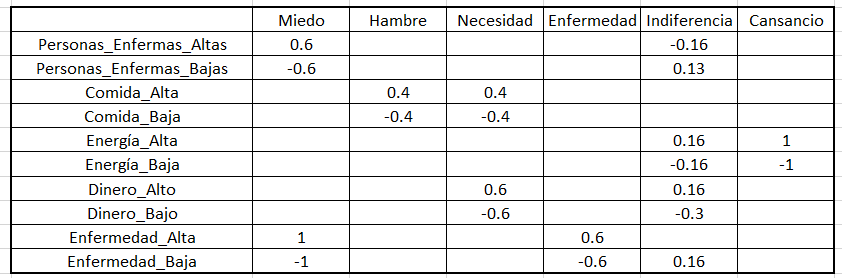
\includegraphics[width=0.9\textwidth]{Graphics/Pesos_Perc_Sent.png}
    \caption{Matriz de adyacencia del grafo de la figura 2.6 con los pesos de las aristas.}
\end{figure}

Una vez obtenidos los grados de pertenencias de los parámetros a los conceptos de $percepci$ó$n$ se procede 
a encontrar los valores sigmoides de los conceptos de $sentimientos$. Se ejemplifica a continuación la dinámica
para encontrar el valor del concepto $Miedo$.
\begin{center}
    Sea $M$ la matriz de adyacencia de la figura 2.6.\\
    Sea $n$ el número total de filas de $M$.\\
    Sea $x$ el valor sigmoide del concepto $Miedo$ y $m$ la columna que representa a $Miedo$ en la matriz.\\
    $\Rightarrow x = \frac{1}{1+ exp(-t)}$ siendo $t = \displaystyle\sum_{i=0}^{n}M[i,m]\times oldConcept$ con $oldConcept$
    representando el valor anterior del concepto i-ésimo.
\end{center}

De esta manera se obtienen los valores correspondientes a los conceptos de $sentimientos$. Este procedimiento
es efectuado tres veces, ya que en cada una se actualizan los $oldConcept$, logrando con esto tener en 
cuenta como se sentía la persona en su acción anterior\footnote{pues en la primera instancia el $oldConcept$
tiene los valores finales de la última acción realizada} y en el momento actual (ya que luego de una iteración
se consiguen los valores correspondientes al instante de tiempo en que se encuentra).

De la misma forma en que se calculan los valores sigmoides de los conceptos de $sentimientos$ se 
calculan los de los conceptos de $acciones$, utilizando a los primeros de la misma forma en que ellos
utilizan a las percepciones.
%Decir los pesos relacionados con las aristas y como estos participan en la toma de decisiones.
\begin{figure}[htb]
    \centering
    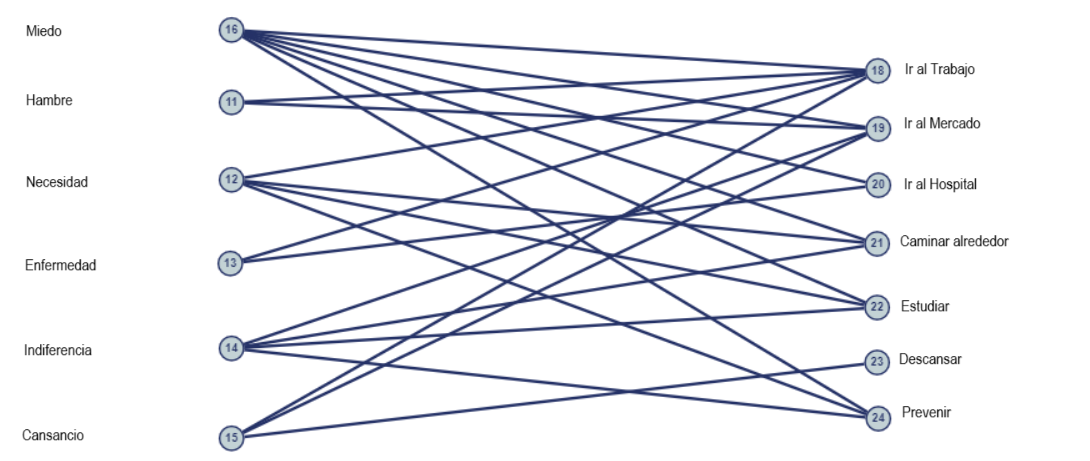
\includegraphics[width=0.9\textwidth]{Graphics/Grafo_Sent-Acciones.png}
    \caption{Grafo que representa las relaciones entre los nodos de $sentimientos$ y $acciones$ del $FCM$ inicial de cada persona}
\end{figure}

\begin{figure}[htb]
    \centering
    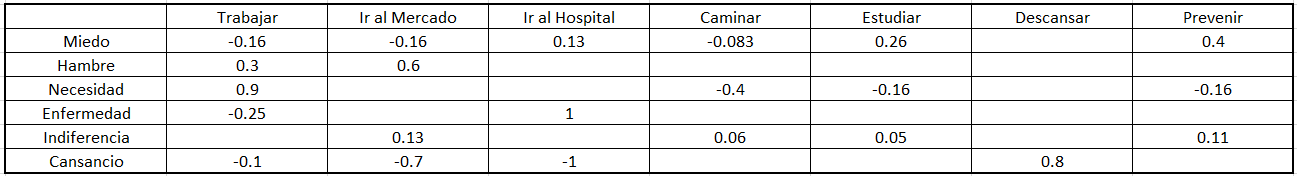
\includegraphics[width=0.9\textwidth]{Graphics/Pesos_Sen_acc.png}
    \caption{Matriz de adyacencia del grafo de la figura 2.8 con los pesos de las aristas.}
\end{figure}

Al obtener los pesos o valores sigmoides correspondientes a los conceptos de $acciones$, el agente que 
representa a la persona en la simulación solo le queda decidir que acción realizar. Para esto se tiene en 
cuenta que no siempre, un ser humano escoge la mejor decisión. Cada $acci$ó$n$ tiene un valor, y es poco
probable que existan varias acciones con el mismo valor asociado, por tanto, en la mayoría de los casos,
existe una acción que en teoría, es mejor que el resto. Entonces, si existe una $acci$ó$n$ que es $"mejor"$
que las otras, ¿qué idea seguir para no escoger siempre esa, pero sí darle más probabilidad de ser escogida?

Primeramente se halla la suma de todos los conceptos de $acciones$ y este resultado es divido por cada uno de 
estos, con el objetivo de hallar la parte que representa cada nodo del total de nodos. Estas cifras son
situadas en una recta numérica, se escoge un número aleatorio entre 0 y 1 y se selecciona, con respecto 
a este número, el primer mayor ubicado en la recta y el primer menor, es decir se escogen los extremos
del intervalo al que pertenezca. Luego, aleatoriamente se selecciona uno de estos dos valores teniendo
la misma probabilidad de ser escogidos, el concepto de $acci$ó$n$ al que este valor hacía referencia, sería
la acción que realizaría el agente en ese momento de la simulación.
%aqui puedo poner un ejemplo de la recta numerica con el random escogido

Los acápites de estas secciones mostraron los pasos que sigue el modelo para representar las acciones
determinantes de las personas en una sociedad que podría estar afectada por una epidemia, por ejemplo: buscar 
atención médica, tomar medidas preventivas y participar en actividades que pueden influir en la propagación 
de la infección. Al igual que los humanos los vectores tienen acciones específicas que modelan su 
comportamiento en relación con la transmisión de la enfermedad. ¿Cuáles son estas acciones y como representarlas?



\section{Vectores y sus acciones}
El enfoque principal brindado a la simulación para los vectores es la acción de picar o no picar. Por esto
los vectores no poseen un $FCM$ como el de las personas, pero siguen siendo agentes en nuestra simulación
pues tiene la posibilidad de decidir si alimentarse o no. En lugar de poseer un $FCM$ se da prioridad a la 
captura de la esencia de la toma de decisiones de los mosquitos en relación con la alimentación.

Estos tienen un parámetro que representa el nivel de saciedad que poseen, en dependencia del valor que este
refleje en el instante de tiempo en que se encuentre, el agente toma la decisión de picar o no, y a cuantas 
personas intentar hacerlo. Decididas la cantidad de personas a picar se genera un valor aleatorio el cual 
se encarga de representar si el vector tuvo éxito en su misión de alimentarse y sin importar el resultado 
obtenido, se continua para la otra persona seleccionada a picar y se repite el proceso.

Es utilizada una población de vectores que no tienen la capacidad de reproducirse, pero si la de morir. Un vector
solo puede morir con la acción de prevenir de una persona, esto es modelado de esta forma para contrarrestar
el hecho de que no pueden procrear. La idea es mantener una población constante, a menos que la sociedad
comience a tomar medidas preventivas.

Todos los procesos relacionados con el picar, infectar o infectarse de los vectores se consideran estocásticos. 
Estos procesos dependen de valores aleatorios que introducen incertidumbre en el 
comportamiento de los vectores. La aleatoriedad se utiliza para capturar la variabilidad inherente en 
la respuesta de los vectores a factores ambientales, biológicos y de interacción con otros organismos.

Cada vez que se realiza una simulación, se generan valores aleatorios que influyen en la toma de decisiones de 
los vectores. Estos valores aleatorios pueden representar la probabilidad de picar a un huésped, la 
probabilidad de transmitir una enfermedad o la probabilidad de ser infectado por un patógeno. Al introducir 
esta aleatoriedad, se logra representar la realidad y se pueden explorar diferentes escenarios 
y resultados posibles.

Es importante destacar que el uso de valores aleatorios en los procesos relacionados con los vectores en la 
simulación no implica que los resultados sean impredecibles, la idea es reflejar la 
naturaleza probabilística de estos procesos en un entorno.

Las acciones de vectores y la de los humanos son de importancia modelar, pues el comportamiento de los 
agentes en caso de epidemia es vital para evitar la propagación de la misma. Sin embargo teniendo una modelación
de las acciones no es suficiente, es necesario indagar sobre la probabilidad de transmisión de la enfermedad en 
cuestión y la probabilidad de infección de los agentes, para cuando estos realicen sus labores diarias
la transmisión se asemeje a la realidad de esta.

\section{Infección, muerte y recuperación de los agentes}
De los principales aspectos en la simulación se encuentran el modelado de las muertes y las infecciones.
Estos dos fenómenos son de suma importancia para comprender y predecir la propagación de enfermedades 
transmitidas por vectores, ya que no solo se tiene en cuenta la infección y muerte del humano, sino también
la de los vectores. Para lograr representar estos fenómenos, se utilizan varios
factores, como la transmisión de patógenos, la susceptibilidad de los individuos y la interacción entre ellos.

El modelo permite evidenciar el proceso de infección y su posterior evolución, así como la ocurrencia de 
las muertes relacionadas con la enfermedad en cuestión. Los parámetros que describen estos sucesos son 
extraídos de datos estadísticos del Dengue; ya que es la enfermedad de este tipo que más afecta a la población 
cubana; pero, ¿cuál es la probabilidad de contraer dengue grave?, ¿qué tasa de letalidad posee el dengue?

Según el Centro de Control y Prevención para Enfermedades\footnote{CDC por sus siglas en inglés} en el artículo 
\autocite{CDC2022} el $5\%$ de los casos de Dengue pueden progresar a grave, y la mortalidad puede llegar
hasta un $13\%$ en pacientes que no tengan tratamientos. La cantidad de personas enfermas en la región de América
durante el $2023$ por Dengue fue de aproximadamente tres millones \footnote{$2997097$ casos reportados hasta el primero
de Julio del $2023$, con el $13\%$ de estos casos reportados como graves}\autocite{WHO2023S}. Durante este 
período se contabilizaron $1302$ muertes con una tasa de mortalidad del $0.04\%$.

El proceso de infección de un agente está definido por las picadas. Se expresa a continuación
cómo se infecta una persona. Luego de transcurrir una hora de simulación
o de llegar a una nueva localización, la persona se sometida a un proceso aleatorio para obtener la 
cantidad de vectores que decidirán picarla\footnote{Cada vector tiene una probabilidad de intentar 
picar del $50\%$}. La ocurrencia o no del hecho de picar, depende también de un valor aleatorio, el cual es 
definido por el usuario de la aplicación en el momento de su uso, al igual que la probabilidad de infectarse
en cada picadura.

En el proyecto se presenta una escala del $0$ al $10$ que representa cuan enfermo se encuentra una persona, siendo
$10$ la máxima y $0$ la mínima. La máxima infección que puede obtener un agente por una picada es de $5$ en esta 
escala. El hecho de que una persona poseea una infección de $10$ no significa que esta fallezca, en cambio,
el número de infección es multiplicado por un valor que representa la realdiad\footnote{Este valor es escogido 
por el usuario} del proceso para obtener una probabilidad de que el agente en cuestión muera.

\begin{figure}[htb]
    \centering
    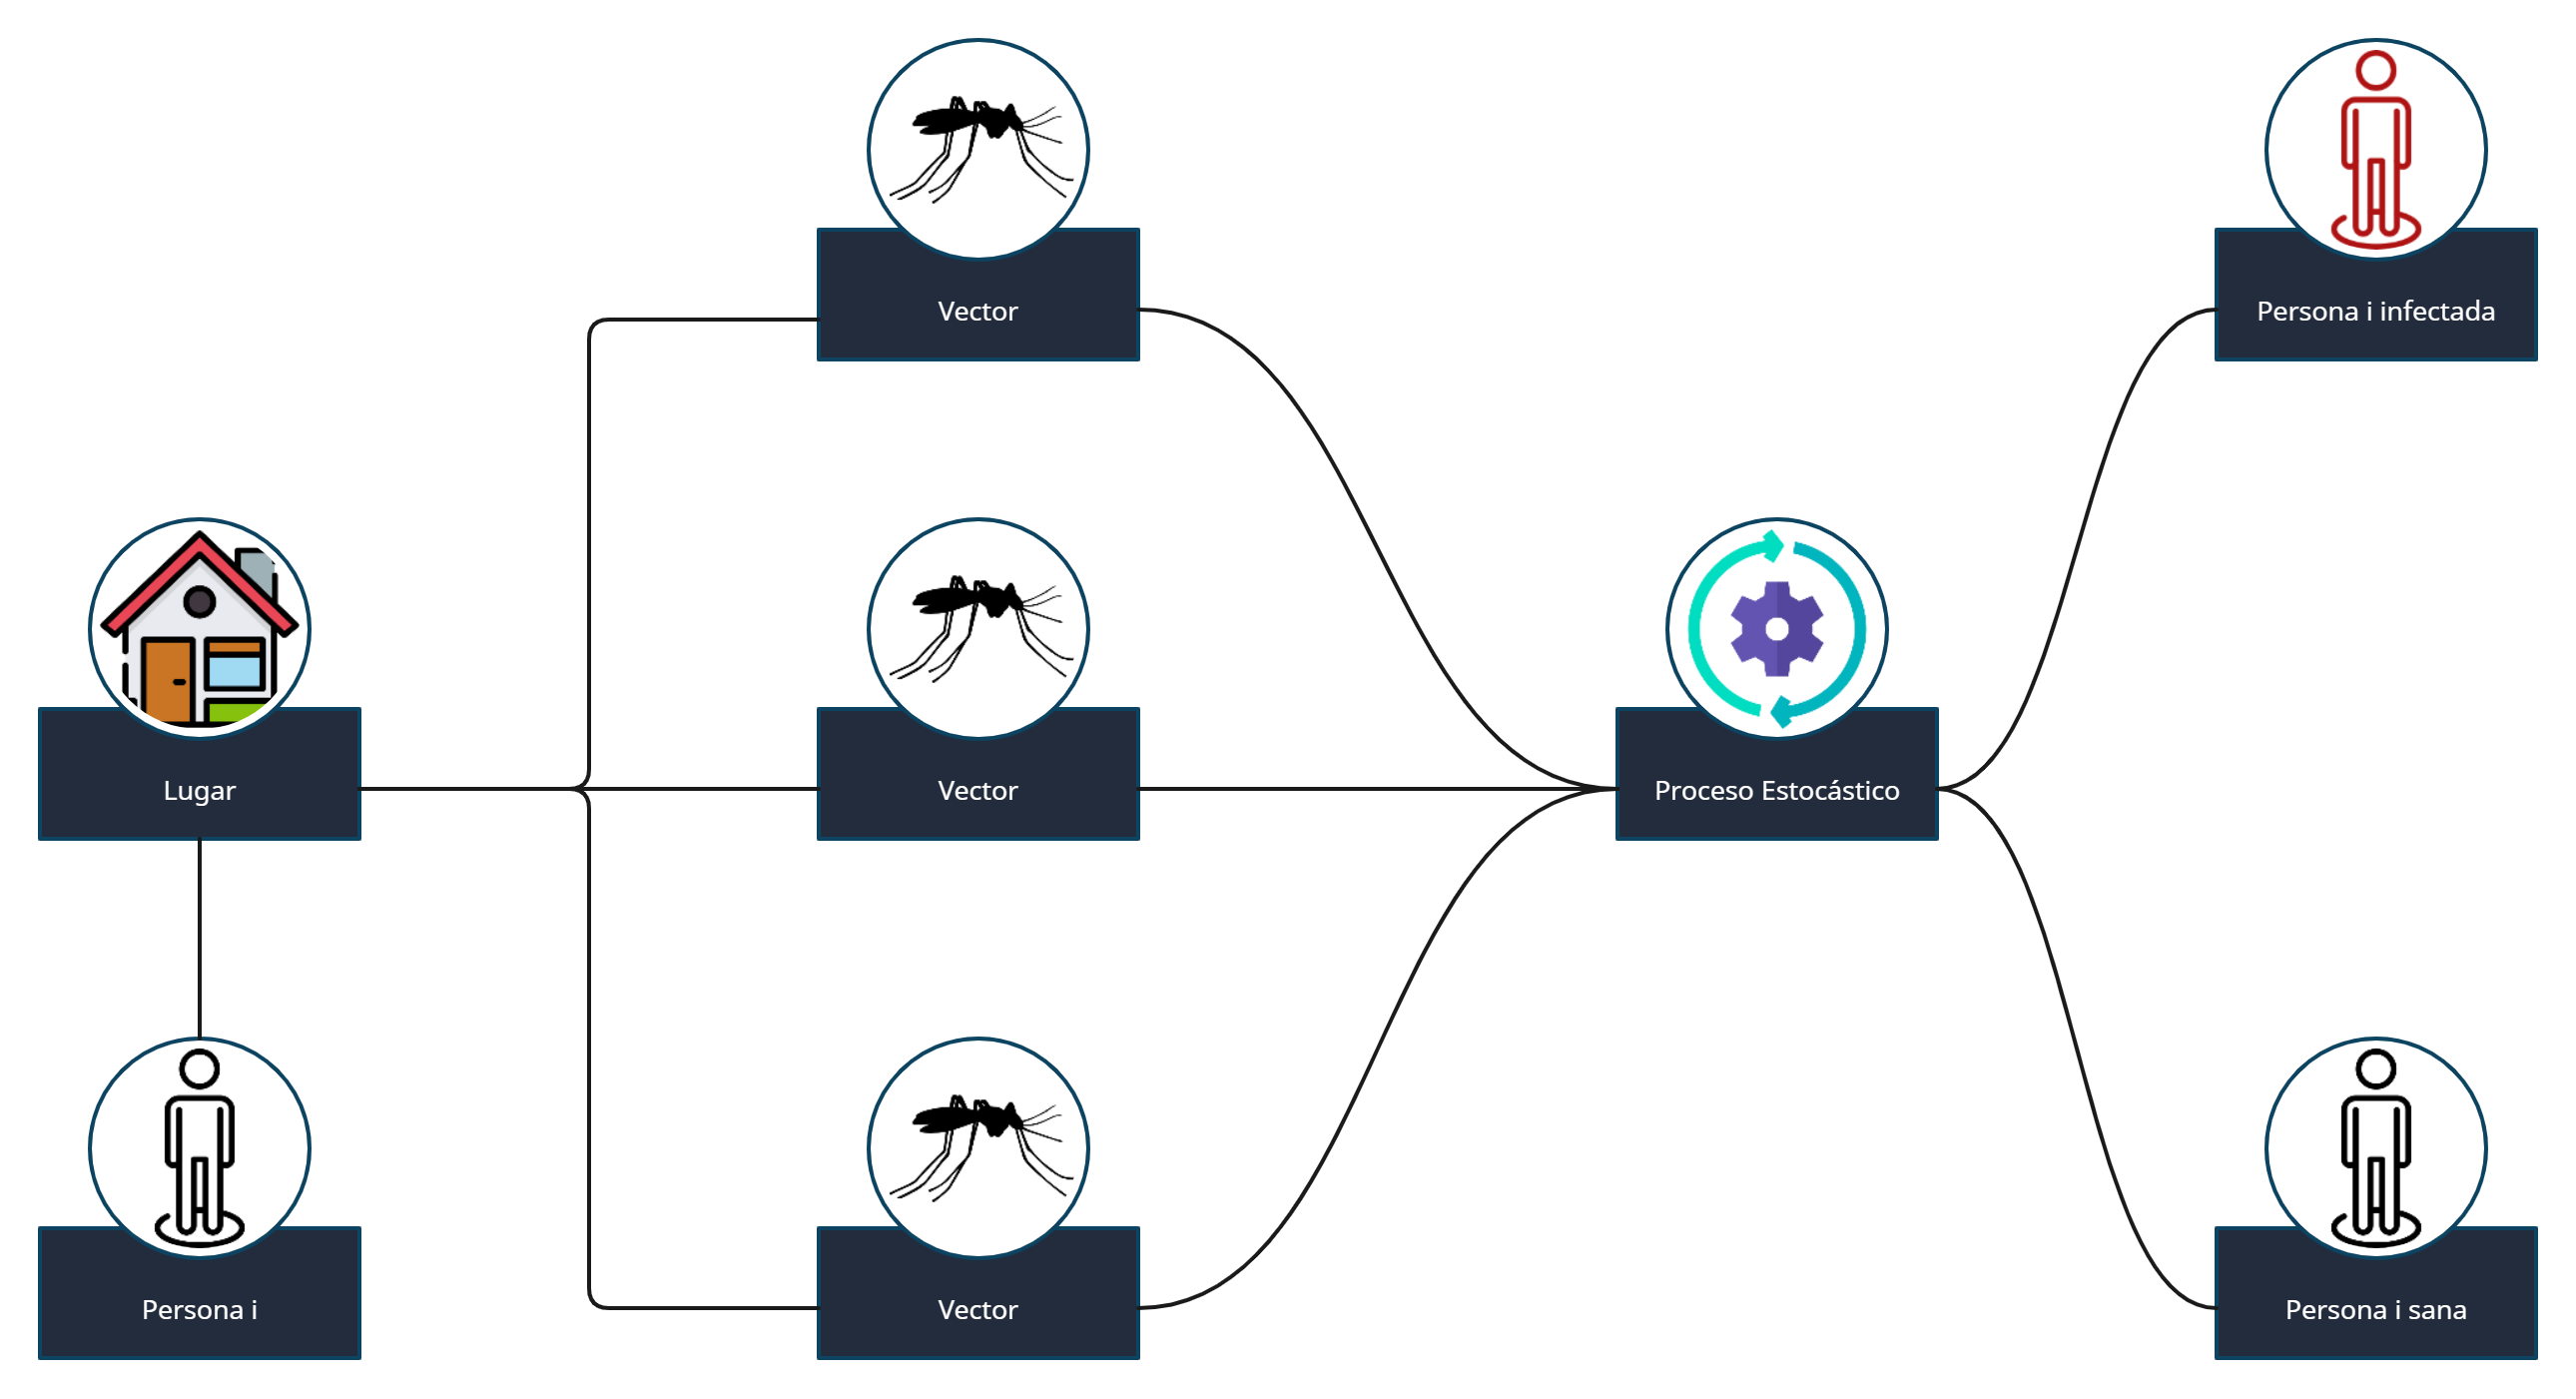
\includegraphics[width=0.9\textwidth]{Graphics/Grafico_Proceso_Picada.jpg}
    \caption{Diagrama que representa el proceso de picar.}
\end{figure}

El caso de los vectores es similar. Al igual que los humanos, estos tienen la misma escala de infección con 
idénticos parámetros e igual probabilidad de infectarse por picada. Al momento de decidir la muerte o no
de un vector se siguen las mismas reglas, pero en caso de muerte, se remplaza el agente por uno nuevo, para 
mantener constante la población de los mismos.
En cuanto al proceso de recuperación, los vectores no tienen la capacidad de recuperarse. En caso de 
fallecimiento, son reemplazados por otro vector de la misma especie. Sin embargo, las personas tienen la 
posibilidad de recuperarse, ya sea mediante atención médica en un hospital o de forma natural. Estos estados 
de recuperación de las personas se modelan nuevamente de manera estocástica, es decir, teniendo en cuenta la 
incertidumbre y variabilidad inherente.

\newpage
\begin{figure}[htb]
    \centering
    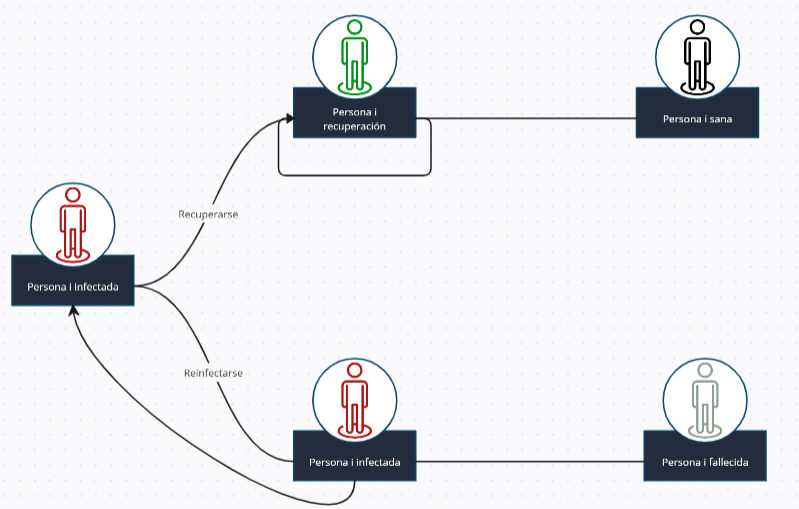
\includegraphics[width=0.8\textwidth]{Graphics/Diagrama_Recuperacion.png}
    \caption{Diagrama que representa el proceso de recuperación.}
\end{figure}


La probabilidad de que una persona se recupere está vinculada a su estado de infección previo al momento en 
que se evalúa este parámetro. Si una persona estaba en proceso de recuperación, es decir, ha disminuido su 
nivel de infección en comparación con el último registro, es más probable que continúe en la fase de 
recuperación. Por otro lado, si el proceso infeccioso estaba en curso, la persona tiene dos posibilidades: 
o bien aumentar los niveles de afectación o bien comenzar a recuperarse.




% "people_sick_high" : (0, 1.4),
%             "people_sick_low" : (1, 1.4),
%             "food_high" : (2, 1.5),
%             "food_low" : (3, 1.5),
%             "energy_high" : (4, 3),
%             "energy_low" : (5, 3),
%             "money_high" : (6, 1.5),
%             "money_low" : (7, 1.5),
%             "sickness_high" : (8, 3.2),
%             "sickness_low" : (9, 3.2)

% "fear" : 10,
%             # "loneliness" : 11,
%             "hunger" : 12,
%             "necessity" : 13,
%             "disease" : 14,
%             "indifference" : 15,
%             "tiredness" : 16


% "go_to_work" : 17,
%             "go_to_market" : 18,
%             "go_to_hospital" : 19,
%             "go_around" : 20,
%             "study" : 21,
%             "rest" : 22,
%             "prevent": 23